\documentclass{article}

\usepackage{xr-hyper}
\usepackage{corl_2026} % Initial submission (anonymous, line numbers).
% \usepackage[final]{corl_2026}
% \usepackage[preprint]{corl_2026}

\usepackage{amsmath,amssymb,amsthm,mathtools}
\usepackage{booktabs,multirow}
\usepackage{graphicx}
\usepackage{xcolor}
\usepackage{xspace}
\usepackage{enumitem}
\usepackage{subcaption}
\usepackage{tikz}
\usetikzlibrary{arrows.meta,positioning,calc,fit,backgrounds,shapes.geometric,decorations.pathreplacing}
\usepackage{pgfplots}
\pgfplotsset{compat=1.18}
\usepgfplotslibrary{groupplots,fillbetween}
\usepackage[capitalise,nameinlink]{cleveref}

% ---------------------------------------------------------------- macros
\newcommand{\method}{\textsc{Cira}\xspace}
\newcommand{\E}{\mathbb{E}}
\newcommand{\R}{\mathbb{R}}
\newcommand{\novel}{\star}
\newcommand{\Pd}{\mathcal{C}^{\delta}_t}
\newcommand{\ind}{\mathbf{1}}
\DeclareMathOperator{\VOI}{VOI}

% Placeholder numbers: every unmeasured value is marked with \ph{...}
% so it can be found with `grep -n '\\ph{' sections/*.tex figures/*.tex`.
\newcommand{\ph}[1]{\textcolor{red!70!black}{#1}}
\newcommand{\phnote}{\textcolor{red!70!black}{\scriptsize placeholder data}}

% Theorem environments
\newtheorem{theorem}{Theorem}
\newtheorem{proposition}{Proposition}
\newtheorem{lemma}{Lemma}
\newtheorem{corollary}{Corollary}
\newtheorem{observation}{Observation}
\theoremstyle{definition}
\newtheorem{definition}{Definition}
\newtheorem{assumption}{Assumption}
\theoremstyle{remark}
\newtheorem{remark}{Remark}

% Colours shared by all figures
\definecolor{cCira}{HTML}{1F6FB2}
\definecolor{cReset}{HTML}{D1495B}
\definecolor{cFrozen}{HTML}{7A7A7A}
\definecolor{cNoCue}{HTML}{E3A33B}
\definecolor{cOracle}{HTML}{2E8B57}
\definecolor{cCont}{HTML}{8E6CB8}
\definecolor{cMem}{HTML}{DCE9F5}

\setlist{itemsep=1pt,topsep=2pt,leftmargin=*}

\externaldocument{supplement}

\title{Adapting Before Contact:\\Contextual Memory for Frozen World Models}

\author{
  Anonymous Authors\\
  Anonymous Institution\\
  \texttt{anonymous@example.com}
}

\begin{document}
\nolinenumbers
\maketitle

\begin{abstract}
Robots typically adapt learned world models online by correcting their prediction errors. In many manipulation tasks, however, the decisive action is committed before any such error can be observed: a puck is struck once, and a load is lifted with a single initial force. We present \method (Context-Indexed Residual Adapters), which equips a frozen visual world model with a persistent library of Bayesian residual dynamics models and infers from visual cues and deployment history which of them applies \emph{before} contact. A factored prior over the library transfers knowledge to unseen combinations of known surfaces and loads, and the same context belief drives decision-aware probing and a latent safety filter calibrated per memory. We show that first-contact prediction error is bounded by memory accuracy plus the log loss of the context filter, and that memories remain calibrated under uncertain assignments only if they are updated with probabilities fixed before each observation. Across simulated striking, world-model benchmarks and a \ph{1{,}200}-episode real-robot deployment, \method reduces first-contact prediction error by \ph{XX\%} relative to episode-reset adaptation, and most of its gain on recurring conditions stems from recall rather than new learning.
\end{abstract}

\keywords{World models, Online adaptation, Contextual inference, Safe control}

\section{Introduction}\label{sec:intro}

\begin{figure}[t]
\centering
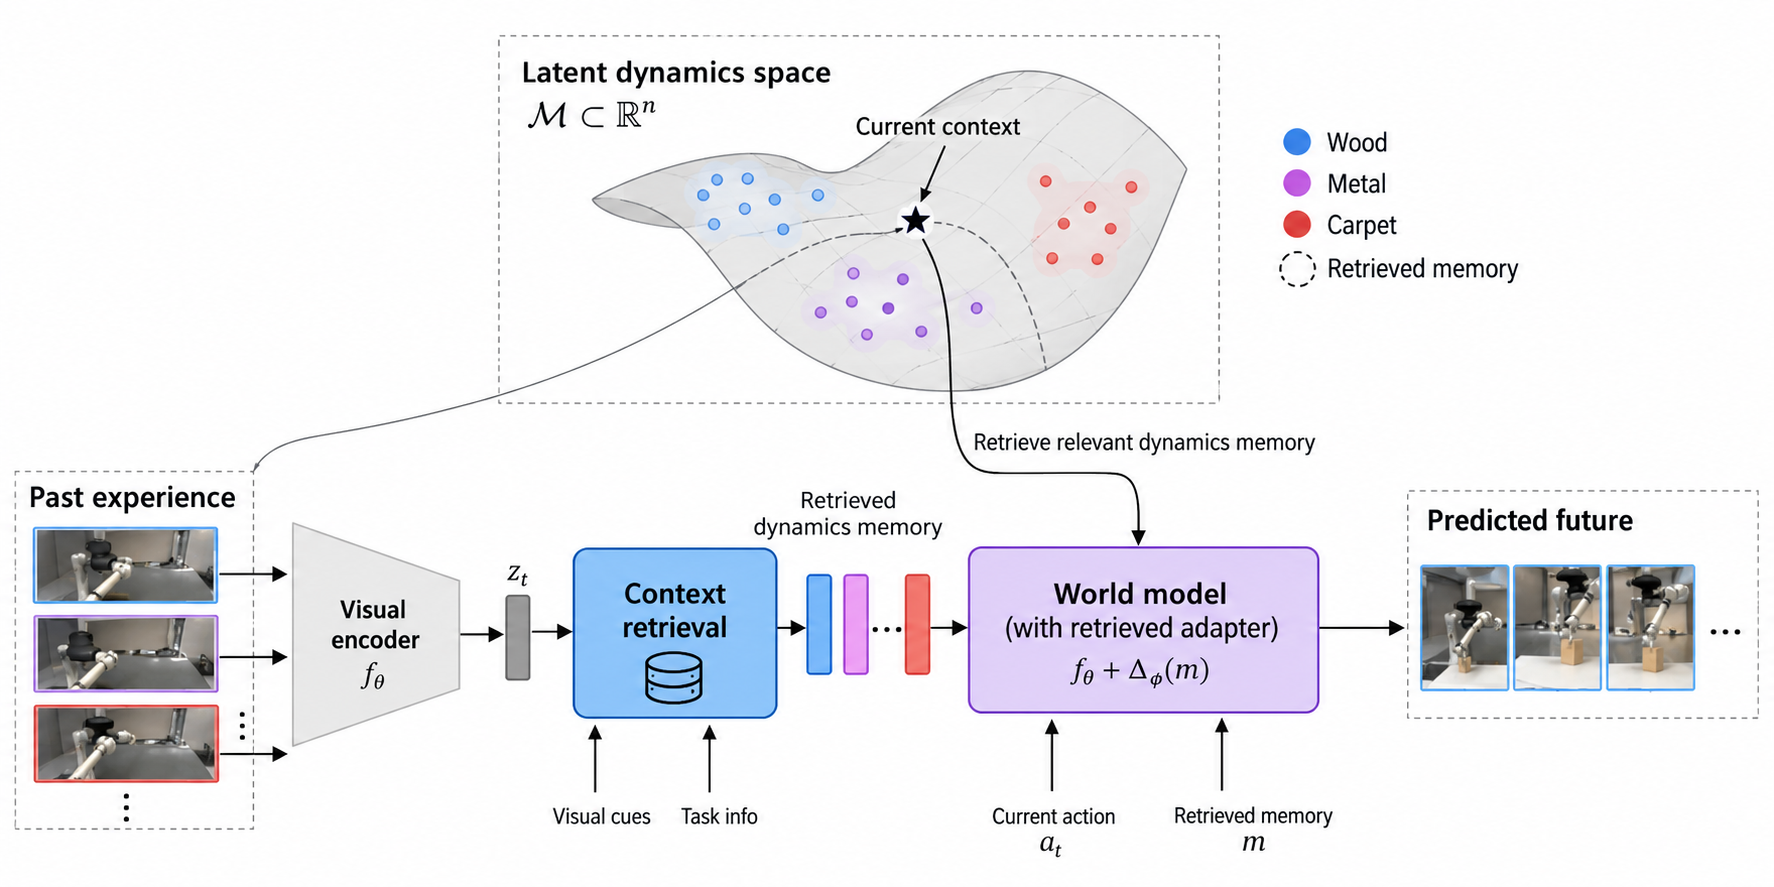
\includegraphics[width=0.92\linewidth]{figures/img/headline.png}
\caption{\textbf{Overview of \method.} A frozen visual world model is augmented with dynamics memories learned during deployment, one per physical context. From visual cues, context retrieval infers which memories apply \emph{before} any interaction, and the retrieved memory corrects the frozen prediction ($f_\theta+\Delta_\phi(m)$ in the figure; $f+\sum_c\pi_e(c)\,m_c$ in \cref{sec:method}).}
\label{fig:headline}
\end{figure}


Visual world models trained on large offline datasets can now plan manipulation tasks directly from images~\citep{zhou2025dinowm,assran2025vjepa2,sobal2025pldm}. Once deployed, however, a robot meets physical conditions its model was never trained on: the same puck slides farther on acrylic than on felt, and a container may be empty or full. A natural remedy is to adapt the model online from its own prediction errors, either by fine-tuning its layers inside the planning loop~\citep{wang2026adajepa} or by training lightweight residual modules around a frozen predictor~\citep{soni2026sandwich}.

This remedy, however, is limited by timing. Consider a robot that must strike a puck so that it stops at a target near a table edge (\cref{fig:teaser}). The correct strike depends on friction and mass, yet the prediction error that would reveal them is observed only after the strike has been executed. Adapting the model at that point improves the next attempt but cannot rescue the current one. Tossing~\citep{zeng2020tossingbot}, the initial force of a lift, and pushing close to an edge share this structure. On such \emph{single-contact tasks}, any scheme driven solely by current-episode errors makes exactly the frozen model's prediction at the moment that matters, however quickly it adapts afterwards (\cref{obs:first}).

Useful information is nevertheless often available before contact, because deployments are repetitive. A robot in a lab or warehouse encounters the same few surfaces, containers and tools many times, and they usually look different from one another. Humans exploit this structure: they maintain separate motor memories for different contexts, recall rather than relearn them when a context returns, and use sensory cues to select the appropriate memory before moving~\citep{heald2021coin,haruno2001mosaic}. This suggests treating adaptation as inference over which known context is active, with learning reserved for new ones.

We instantiate this idea in \method, a module that attaches to any frozen visual world model (\cref{fig:headline}). \method maintains a library of compact Bayesian linear models of the world model's residual error, one per discovered context. Before contact, a context belief combines the frequency of past contexts with visual cues whose association to each memory is learned from dynamics alone. After contact, residuals refine the belief or trigger a new memory. A factored Gaussian prior couples memories that share a surface or a load, so a surface seen with one load and a load seen on another surface jointly predict their unseen combination. The same belief decides whether a diagnostic probe is worth its cost and recalls a safety margin calibrated separately for each memory.

A memory weighted by the posterior computed \emph{after} each residual preferentially absorbs residuals it already explains and becomes biased. \method therefore weights updates by the probability computed before the observation, which yields an error bound whose cross-context contamination is controlled by the log loss of the context filter (\cref{thm:confidence}); the same log loss bounds the first-contact error (\cref{prop:first}).

We evaluate \method on simulated striking and pushing, on the AdaJEPA benchmark tasks~\citep{wang2026adajepa}, and in a \ph{1{,}200}-episode hardware deployment in which people swap mats and containers on a schedule unknown to the robot. \method reduces first-contact error by \ph{XX\%} relative to the strongest episode-reset baseline, predicts held-out surface--load combinations with \ph{XX\%} lower error than independent memories, and owes \ph{XX\%} of its improvement on recurring conditions to recall. Our contributions are (i)~a formalization of the first-contact limitation (\cref{sec:problem}); (ii)~\method, a persistent, cue-driven and compositional memory for frozen world models (\cref{sec:method}); (iii)~bounds on memory, first-contact and decision error and an identifiability condition for unseen combinations (\cref{sec:analysis}); and (iv)~experiments showing that recall, rather than faster optimization, accounts for most of the gain (\cref{sec:experiments}).


\section{Related Work}\label{sec:related}

\paragraph{Adapting world models at deployment.}
Test-time training adapts a model with self-supervised losses on incoming data~\citep{sun2020ttt,wang2021tent}. For latent world models~\citep{hafner2025dreamerv3,hansen2024tdmpc2,zhou2025dinowm}, AdaJEPA applies it within the planning loop~\citep{wang2026adajepa} and Sandwich-Residuals restricts it to residual modules around a frozen predictor~\citep{soni2026sandwich}. Both reset at every episode, and continual variants that never reset are known to degrade on long, recurring streams~\citep{wang2022cotta,press2023rdumb,hoang2024petta}. Meta-learned adaptation~\citep{nagabandi2018learning,kumar2021rma} and contextual world models~\citep{lee2020context,roder2025dali,benad2026dmash} infer a continuous context from recent transitions, which also requires interaction.

\paragraph{Mixtures of dynamics models.}
MOLe maintains a persistent mixture of dynamics models under a Chinese restaurant process prior~\citep{nagabandi2019mole}. Related approaches use Dirichlet- and Gaussian-process mixtures~\citep{xu2020taskagnostic,jerfel2019reconciling,lee2020cndpm}, changepoint detection over Bayesian last layers~\citep{harrison2018alpaca,harrison2020moca}, or switching dynamical systems~\citep{fox2011bnpslds,linderman2017rslds}. All select a context from prediction error alone and treat contexts as unstructured. \method adds cue-based selection before contact and shares statistical strength across the factors of a context. In human motor learning, the COIN model explains savings and cue effects through the same kind of inference~\citep{heald2021coin,heald2023annurev}; we adopt its distinction between \emph{apparent} and \emph{proper} learning as a measurement.

\paragraph{Anticipating dynamics from vision and latent safety.}
Terrain-aware models~\citep{gibson2024visualterrain,agarwal2022egocentric,brunzema2026vcvbll}, image-to-property maps supervised by proprioception~\citep{loquercio2022crossmodal,margolis2023activesensing} and vision-language priors~\citep{gao2024physically,wang2026phys2real} map appearance to a continuous physical quantity through a fixed channel; \method maps appearance to self-discovered contexts and lets dynamics evidence overrule it. Latent safety filters apply reachability or barrier functions in a world model's latent space~\citep{nakamura2025latent,nakamura2026latentcbf,seo2025uncertainty}, and adaptive conformal inference~\citep{gibbs2021adaptive} has been combined with such filters and latent MPC~\citep{huriot2026safe,nath2026pixels}. These methods calibrate a single model, whereas \method stores one calibration per memory.

\section{Problem Formulation}\label{sec:problem}

% First-contact timeline (compact).
\begin{figure}[t]
\centering
\resizebox{\linewidth}{!}{%
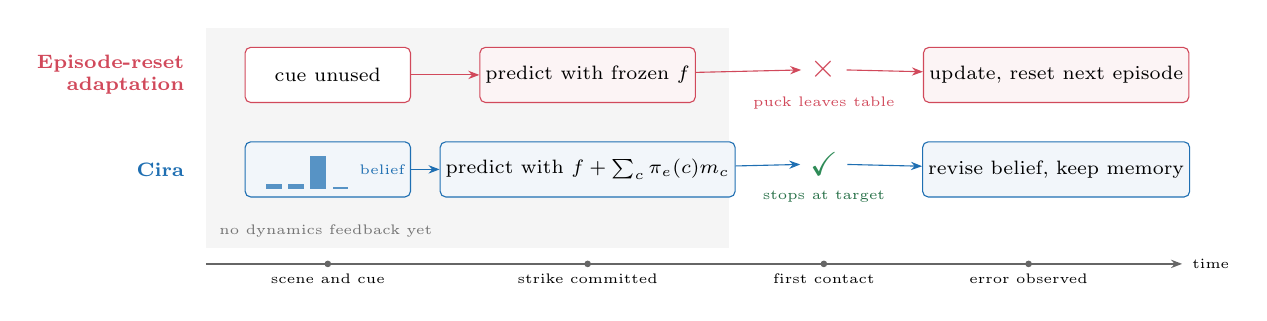
\begin{tikzpicture}[
  font=\scriptsize,
  >={Stealth[length=4pt]},
  box/.style={draw, rounded corners=2pt, minimum height=7mm, minimum width=21mm, inner sep=2pt, align=center},
  lane/.style={font=\scriptsize\bfseries, anchor=east, align=right},
]
\def\xa{1.45}\def\xb{4.75}\def\xc{7.75}\def\xd{10.35}
\fill[black!4] (-0.1,-1.75) rectangle (6.55,1.05);
% lane 1: reset
\node[lane, text=cReset] at (-0.25,0.45) {Episode-reset\\adaptation};
\node[box, draw=cReset, fill=white] (r0) at (\xa,0.45) {cue unused};
\node[box, draw=cReset, fill=cReset!6] (r1) at (\xb,0.45) {predict with frozen $f$};
\node[font=\large, text=cReset] (rx) at (\xc,0.52) {$\times$};
\node[font=\tiny, text=cReset, anchor=north] at (\xc,0.3) {puck leaves table};
\node[box, draw=cReset, fill=cReset!6] (r2) at (\xd+0.35,0.45) {update, reset next episode};
\draw[->, cReset] (r0) -- (r1); \draw[->, cReset] (r1) -- (rx); \draw[->, cReset] (rx) -- (r2);
% lane 2: CIRA
\node[lane, text=cCira] at (-0.25,-0.75) {\method};
\node[box, draw=cCira, fill=cCira!6] (c0) at (\xa,-0.75) {};
\begin{scope}[shift={(\xa-0.78,-1.0)}]
  \foreach \i/\h in {0/0.07, 1/0.06, 2/0.42, 3/0.03} {
    \fill[cCira!75] (\i*0.28,0) rectangle ++(0.2,\h);
  }
\end{scope}
\node[font=\tiny, text=cCira, anchor=west] at (\xa+0.28,-0.75) {belief};
\node[box, draw=cCira, fill=cCira!6] (c1) at (\xb,-0.75) {predict with $f+\sum_c\pi_e(c)m_c$};
\node[font=\large, text=cOracle] (cx) at (\xc,-0.68) {$\checkmark$};
\node[font=\tiny, text=cOracle!80!black, anchor=north] at (\xc,-0.9) {stops at target};
\node[box, draw=cCira, fill=cCira!6] (c2) at (\xd+0.35,-0.75) {revise belief, keep memory};
\draw[->, cCira] (c0) -- (c1); \draw[->, cCira] (c1) -- (cx); \draw[->, cCira] (cx) -- (c2);
% time axis
\draw[->, thick, black!60] (-0.1,-1.95) -- (12.3,-1.95) node[right, black, font=\tiny] {time};
\foreach \x/\t in {\xa/{scene and cue}, \xb/{strike committed}, \xc/{first contact}, \xd/{error observed}} {
  \fill[black!60] (\x,-1.95) circle (1.2pt);
  \node[below=0pt, font=\tiny] at (\x,-1.95) {\t};
}
\node[font=\tiny, text=black!55, anchor=south west] at (-0.05,-1.73) {no dynamics feedback yet};
\end{tikzpicture}}
\caption{\textbf{The first-contact limitation.} The strike is committed before any dynamics error is observed (shaded), so an episode-reset adapter strikes with the frozen model; \method selects memories before the strike.}
\label{fig:teaser}
\end{figure}


We consider a frozen encoder and predictor that map an observation $o_{e,t}$ and action $a_{e,t}$ at step $t$ of episode $e$ to $z_{e,t}=E(o_{e,t})\in\R^d$ and $\hat z_{e,t+1}=f(z_{e,t},a_{e,t})$. Each episode is governed by an unobserved physical context $c_e$, such as ``acrylic mat, heavy puck,'' which remains fixed within the episode. The true latent dynamics are
\begin{equation}\label{eq:dynamics}
  z_{e,t+1}=f(z_{e,t},a_{e,t})+\mu_{c_e}(z_{e,t},a_{e,t})+\epsilon_{e,t},\qquad \E[\epsilon_{e,t}\mid z_{e,t},a_{e,t},c_e]=0,
\end{equation}
where $\mu_c$ denotes the mean residual of context $c$ relative to the frozen model, with $\mu_0\equiv0$ for the training condition, and the noise may depend on state and action. The robot observes episode boundaries but never context labels, and it may retain memories across episodes. Before its first informative interaction it extracts a visual cue $y_e$ from the scene. We write $D_{<e}$ for all data observed before episode $e$ and assume that the approach motion reveals nothing about $c_e$ beyond $y_e$ and $D_{<e}$.

\begin{definition}[Single-contact task]\label{def:single}
A task is \emph{single-contact} with respect to an outcome $J^{\mathrm{first}}_e$ if the action determining $J^{\mathrm{first}}_e$ is committed at a step $\tau_e$ before any feedback from its context-dependent transition is available, and no later action can change $J^{\mathrm{first}}_e$.
\end{definition}

In striking, $J^{\mathrm{first}}_e$ is the stopping error of the strike.

\begin{observation}[First-contact initialization]\label{obs:first}
Consider an adaptive predictor whose state changes only in response to current-episode prediction errors. If no such error is available before $a_{e,\tau_e}$ is committed, its prediction at $\tau_e$ equals its prediction at the start of the episode. In particular, a predictor reset to the frozen model at every episode satisfies $\hat z^{\mathrm{adapt}}_{e,\tau_e+1}(z,a)=f(z,a)$ and incurs first-contact bias $\|\mu_{c_e}\|$.
\end{observation}

This holds for any optimizer and adaptation speed, so improvement at the first contact must come from knowledge retained across episodes or from evidence in the scene. Our goal is therefore the pre-contact predictive distribution
\begin{equation}\label{eq:mixture}
  p(z'\mid z,a,y_e,D_{<e})=\textstyle\sum_{c}\pi_e(c)\,p(z'\mid z,a,c,D_{<e}),\qquad \pi_e(c)=p(c_e=c\mid y_e,D_{<e}),
\end{equation}
where the sum also includes a hypothesis for contexts not yet represented in memory.

\section{Method}\label{sec:method}

\method augments a frozen world model with a library of residual memories, a factored prior that relates memories through their physical factors, and a context filter that decides which memory to use and which to update (overview in \cref{fig:method}, \cref{app:impl}). The encoder and predictor are never modified.

\subsection{Residual Memories}
Let $U\in\R^{d\times k}$ with $k\ll d$ contain the leading principal directions of the frozen model's residuals $r_t=z_{t+1}-f(z_t,a_t)$ on training data, and let $\phi(z,a)\in\R^p$ be a fixed feature map such as $[a,\,U^\top z,\,1]$. Memory $c$ models each coordinate of the projected residual $v_t=U^\top r_t$ as a Bayesian linear regression,
\begin{equation}\label{eq:adapter}
  v_{t,i}\mid c,w_{c,i}\sim\mathcal N\big(w_{c,i}^\top\phi_t,\ \sigma_i^2(z_t,a_t)\big),\qquad i=1,\dots,k,
\end{equation}
which admits closed-form updates~\citep{harrison2018alpaca}. Its latent correction is $m_c(z,a)=U\widehat W_c\phi(z,a)$, where $\widehat W_c$ stacks the posterior means. Including the action in $\phi$ lets a memory represent friction or gain changes whose effect scales with the action. The noise scale $\sigma_i(z,a)$ is a small network fitted to training residuals~\citep{kersting2007hetgp}. It is large during impacts and stick--slip, where the frozen model is least accurate, which prevents contact transients from being mistaken for a change of context~\citep{bauza2017probpush}.

\subsection{A Factored Prior for Unseen Combinations}
We represent a context as a tuple of factor values $c=(c^1,\dots,c^F)$, for instance a surface and a load. The prior correlates memories that share factor values,
\begin{equation}\label{eq:kernel}
  \operatorname{Cov}(w_{c,i},w_{c',i})=k_{\mathcal C}(c,c')\,\Sigma_0,\qquad
  k_{\mathcal C}(c,c')=\kappa_0^2+\textstyle\sum_{j=1}^{F}\kappa_j^2\,\ind\{c^j=c'^j\}+\kappa_\times^2\,\ind\{c=c'\}.
\end{equation}
This separable multi-output kernel~\citep{alvarez2012kernels} has a shared term, one term per factor and an interaction term. Conditioning on the stored memories yields a prior mean and variance for every unseen tuple before its first contact, and $\kappa_\times>0$ preserves uncertainty about interactions that no other combination can reveal. Factor roles and image regions (table surface, object crop) are specified; factor values are discovered from dynamics without labels.

\subsection{Context Inference Before and After Contact}
Let $q_t(c)$ denote the context probability immediately before the residual $v_t$ is observed, and $\pi_t^+(c)$ the probability immediately after. At the start of an episode the belief combines history and cues, and it is then updated with each transition:
\begin{equation}\label{eq:cue}
  q_{\tau_e}(c)=\pi_e(c)\ \propto\ p(c\mid D_{<e})\textstyle\prod_{j}p_\eta(y^j_e\mid c^j),\qquad
  \pi_t^+(c)\ \propto\ q_t(c)\,p(v_t\mid z_t,a_t,c),
\end{equation}
with $q_{t+1}=\pi_t^+$ within an episode. The history prior $p(c\mid D_{<e})$ is a sticky Chinese restaurant process~\citep{fox2011sticky} that reserves probability mass for new factor values, and a new memory is instantiated when this hypothesis remains the most probable for several consecutive steps. Each cue model $p_\eta(y^j\mid c^j)$ is a Gaussian over a low-dimensional projection of the encoder features in the corresponding image region. Cue models are trained on beliefs from a parallel filter that ignores the cue, so a cue is never reinforced by its own predictions and a misleading association is gradually unlearned.

\subsection{Learning From Uncertain Assignments}
Each memory is updated with the \emph{predictive} probability $q_t$ rather than the filtered probability $\pi_t^+$:
\begin{equation}\label{eq:update}
  \omega_{c,i,t}=\tfrac{q_t(c)}{\sigma_i^2(z_t,a_t)},\ \
  V_{c,i,t}=P_{c,i}+\sum_{s<t}\omega_{c,i,s}\phi_s\phi_s^\top,\ \
  \widehat w_{c,i,t}=V_{c,i,t}^{-1}\Big(P_{c,i}\nu_{c,i,t}+\sum_{s<t}\omega_{c,i,s}\phi_s v_{s,i}\Big),
\end{equation}
where $\nu_{c,i,t}$ is the prior mean implied by \cref{eq:kernel} and $P_{c,i}$ is the prior precision fixed at creation. The distinction matters because a weight computed from the current residual favours residuals that the memory already predicts well; the memory then learns from truncated noise and becomes biased (\cref{rem:bias}). Predictive weights keep the noise zero-mean given the weight, which our analysis requires.

\subsection{Planning, Probing, and Safety}
\paragraph{Planning and probing.}
The planner rolls out each memory's correction and minimizes the belief-weighted cost $\widehat J_e(a)=\sum_c\pi_e(c)\widehat J_c(a)$ over candidate actions with the cross-entropy method~\citep{rubinstein1999cem,chua2018pets}. When the task permits a diagnostic probe, such as a gentle nudge, \method executes it only if its value of information for the subsequent decision exceeds its cost; this value vanishes when all plausible contexts call for the same strike (\cref{app:voi}).

\paragraph{Per-memory safety margins.}
Given a latent safety function $h$ with $h\ge0$ on safe states~\citep{nakamura2026latentcbf}, the filter accepts an action only if the discrete-time barrier condition~\citep{agrawal2017discrete}
\begin{equation}\label{eq:cbf}
  h(\bar z'_{c,t})-L_h\,b_{c,t}\ \ge\ (1-\alpha)\,h(z_t),\qquad \bar z'_{c,t}=f(z_t,a_t)+m_c(z_t,a_t),
\end{equation}
holds for every memory in a plausible set $\Pd$ that carries at least $1-\delta$ of the belief, where $b_{c,t}$ is a margin stored with memory $c$. After each transition, the step is attributed to one plausible memory based on its score $s_{c,t}=\|z_{t+1}-\bar z'_{c,t}\|$, and only that margin is updated, $b_{c,t+1}=b_{c,t}+\gamma(\ind\{s_{c,t}>b_{c,t}\}-\delta_s)$; this is adaptive conformal inference~\citep{gibbs2021adaptive} run separately for each memory (details in \cref{app:safety}). When a known context returns, its calibrated margin returns with it.

\section{Theoretical Analysis}\label{sec:analysis}

We bound memory error under uncertain assignments, relate it to the first contact, and characterize composition and safety. All proofs, together with a summary of the results, are given in the supplementary material (\cref{app:summary,app:proofs}).

\begin{assumption}[Realizability and predictable noise]\label{ass:main}
For every context $c$ there is a fixed $W_c$ with $\mu_c(z,a)=UW_c\phi(z,a)$ on the inputs considered, so that $v_t=W_{c_t}\phi_t+\xi_t$. Conditioned on the history up to $(z_t,a_t)$, the cue and the true context $c_t$, each $\xi_{t,i}$ is zero-mean and $\sigma_i(z_t,a_t)$-sub-Gaussian. Contexts and actions may depend adversarially on past data but not on the current noise. We write $\Delta_{\max}=\sup_{c,c',x}\|\mu_c(x)-\mu_{c'}(x)\|$.
\end{assumption}

\subsection{Memory Accuracy Under Uncertain Assignments}

\begin{theorem}[Uniform memory error]\label{thm:confidence}
Under \cref{ass:main}, let memory $c$ be updated by \cref{eq:update} and let $\delta_c\in(0,1)$. With probability at least $1-\delta_c$, simultaneously for all $t$, all $\phi\in\R^p$ and all coordinates $i$,
\begin{equation}\label{eq:thm-conf}
  \big|\phi^\top(\widehat w_{c,i,t}-w_{c,i})\big|\le\beta_{c,i,t}\|\phi\|_{V^{-1}_{c,i,t}},\ \ 
  \beta_{c,i,t}=\textstyle\sqrt{2\log\frac{k}{\delta_c}+\log\frac{\det V_{c,i,t}}{\det P_{c,i}}}
  +\|\nu_{c,i,t}-w_{c,i}\|_{P_{c,i}}+B_{c,i,t},
\end{equation}
where $B^2_{c,i,t}=\sum_{s<t}\omega_{c,i,s}[\phi_s^\top(w_{c_s,i}-w_{c,i})]^2\le\Delta_{\max}^2M_{c,i,t}$ and $M_{c,i,t}=\sum_{s<t:\,c_s\neq c}\omega_{c,i,s}$ is the weight the memory assigned to other contexts. If moreover $\sigma_i\ge\sigma_{\min}$, then
\begin{equation}\label{eq:contam-logloss}
  \textstyle\sum_c M_{c,i,T}\ \le\ \sigma_{\min}^{-2}\sum_{t<T}\big(1-q_t(c_t)\big)\ \le\ \sigma_{\min}^{-2}\sum_{t<T}-\log q_t(c_t).
\end{equation}
\end{theorem}

The three terms of $\beta$ are noise, prior mismatch and contamination. Noise shrinks with data and prior mismatch captures negative transfer, but contamination does not vanish with more data; by \cref{eq:contam-logloss} it is controlled by the step-level log loss of the context filter, so more accurate context prediction directly yields more accurate memories. The proof applies the self-normalized martingale bound of \citet{abbasi2011improved}, which is valid only because $q_t(c)$ is determined before $\xi_t$ is drawn. With filtered weights this step fails; \cref{rem:bias} in the appendix gives a simple example in which the estimate converges to a biased value while its interval shrinks.

\subsection{From Context Prediction to the First Contact}

Let $x_e=(z_{e,\tau_e},a_{e,\tau_e})$ be the first-contact query and $b_e=\|\sum_c\pi_e(c)m_{c}(x_e)-\mu_{c_e}(x_e)\|$ the bias of the pre-contact mixture prediction.

\begin{proposition}[First-contact separation]\label{prop:first}
Suppose the library contains every context that occurs and $\|m_c(x)-\mu_c(x)\|\le\epsilon_e$ for all contexts in the support of $\pi_e$. Then
\begin{equation}\label{eq:first}
  b_e\le\epsilon_e+\big(1-\pi_e(c_e)\big)\Delta_{\max},\qquad
  \textstyle\sum_{e=1}^{N}b_e\le\sum_e\epsilon_e+\Delta_{\max}\sum_e-\log\pi_e(c_e).
\end{equation}
In contrast, an episode-reset predictor has bias $\|\mu_{c_e}(x_e)\|$ by \cref{obs:first}; if this is at least $\Delta_{\min}$ on $N_{\mathrm{shift}}$ episodes, its cumulative bias is at least $N_{\mathrm{shift}}\Delta_{\min}$.
\end{proposition}

The episode-level log loss measures how predictable the context sequence is from history and cues; for a Krichevsky--Trofimov predictor with revealed labels it is at most $N\widehat H(C\mid Y)+O(K|\mathcal Y|\log N)$ for every sequence~\citep{krichevsky1981performance} (\cref{cor:entropy}). Memory thus helps to the extent that contexts recur, and a cue to the extent that it is informative; without recurrence the bound predicts no gain. The result extends to the new-context hypothesis (\cref{cor:novel}) and, for Lipschitz dynamics and costs, to the committed action: the belief-weighted plan is within $2L_\ell C_HH[\bar\epsilon_e+(1-\pi_e(c_e))\Delta_{\max}]$ of the best candidate over horizon $H$ (\cref{cor:decision}).

\subsection{Composition and Safety}

\begin{proposition}[Identifiability of an unseen combination]\label{prop:composition}
Fix one coordinate and one feature vector, and let $g(c)=\phi^\top w_c$ follow the prior \cref{eq:kernel} with $\kappa_0,\kappa_j>0$. Suppose $g$ is known exactly on a set $\Omega$ of observed combinations, and let $q\notin\Omega$ consist of factor values that occur in $\Omega$.
(i)~If $\kappa_\times=0$, the conditional variance of $g(q)$ vanishes if and only if the factor indicators of $q$ lie in the span of those of $\Omega$. For two factors, this holds if and only if the two values of $q$ belong to the same connected component of the bipartite graph whose edges are the observed combinations.
(ii)~If $\kappa_\times>0$, the conditional variance is at least $\kappa_\times^2\,\phi^\top\Sigma_0\phi$, regardless of how many combinations are observed.
\end{proposition}

Observing every factor value is thus not sufficient; the observed combinations must connect them (\cref{fig:theory-composition}).

Finally, if the safety filter is enforced exactly, latent barrier violations after $T$ steps number at most $\delta_sT$ plus a term proportional to the number of memories, for every sequence of contexts and cues, including misleading ones (\cref{app:safety}).

\section{Experiments}\label{sec:experiments}

\subsection{Experimental Setup}

\paragraph{Tasks.}
In \emph{simulation} (MuJoCo), a robot strikes a puck toward a target near a table edge or pushes a box close to an edge, with three surfaces (friction \ph{0.60}, \ph{0.35}, \ph{0.12}) and three loads (\ph{0.2}, \ph{0.6}, \ph{1.0}\,kg); the world model is a DINO-WM-style predictor on frozen DINOv2 features~\citep{zhou2025dinowm} trained on a single condition. On the \emph{benchmarks}, we use PushT and PointMaze with the released AdaJEPA checkpoints~\citep{wang2026adajepa} and pair the existing agent and block recolourings with changes in mass and damping, so that colour becomes an imperfect cue. On \emph{hardware}, a Franka Panda strikes a puck on interchangeable mats and lifts containers of unknown mass using a frozen V-JEPA~2-AC predictor~\citep{assran2025vjepa2}. During a \ph{1{,}200}-episode deployment, lab members exchanged mats and containers on a schedule unknown to the robot.

\paragraph{Protocol and baselines.}
Each stream has $N=\ph{500}$ episodes over $K=9$ surface--load contexts with geometric dwell times. The cue shows the true context's appearance with probability $\rho$ and each other appearance with probability $(1-\rho)/(K-1)$, so $\rho=1/K$ is uninformative. We report 95\% bootstrap intervals over \ph{10} streams shared by all methods, and compare against the \emph{Frozen} world model; \emph{Reset-SGD}, which takes AdaJEPA-style gradient steps and resets every episode~\citep{wang2026adajepa}; \emph{Reset-Residual}, a Sandwich-Residuals-style adapter that also resets~\citep{soni2026sandwich}; \emph{Continual-SGD}, the same updates without resets; \emph{Mixture}, a persistent mixture of dynamics models selected from prediction error alone~\citep{nagabandi2019mole}; \emph{\method-NoCue}, our method without cues; and \emph{Oracle}, which uses \method's memories with the true context. All methods share backbone, planner, candidates and action budget; hyperparameters are tuned on separate development streams.

% PLACEHOLDER DATA: every coordinate in this file is illustrative and must be
% replaced by measured values before submission.
\begin{figure}[t]
\centering
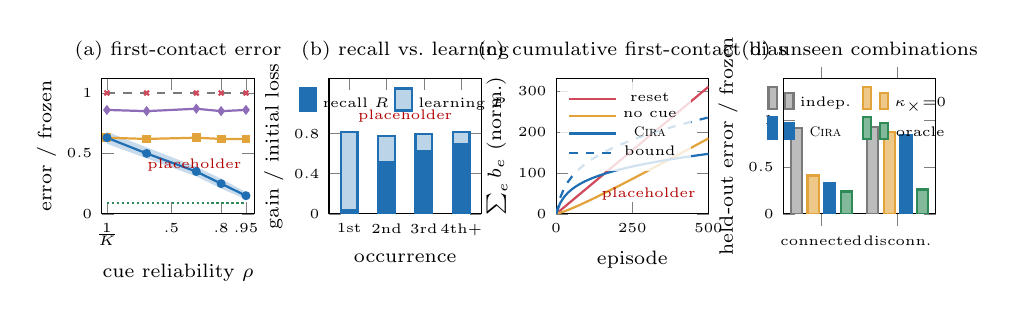
\begin{tikzpicture}
\begin{groupplot}[
  group style={group size=4 by 1, horizontal sep=0.95cm},
  width=0.29\linewidth, height=3.3cm,
  tick label style={font=\tiny}, label style={font=\scriptsize}, title style={font=\scriptsize, yshift=-3pt},
  ylabel style={yshift=-3pt},
  legend style={font=\tiny, draw=none, fill=none},
  every axis plot/.append style={thick, mark size=1.2pt},
]
% ---------------------------------------------------------------- (a) error vs cue reliability
\nextgroupplot[
  title={(a) first-contact error},
  xlabel={cue reliability $\rho$}, ylabel={error / frozen},
  xmin=0.08, xmax=1.0, ymin=0, ymax=1.12,
  xtick={0.11,0.5,0.8,0.95}, xticklabels={$\frac1K$,.5,.8,.95},
  legend to name=leg:results, legend columns=6,
]
\addplot[cFrozen, dashed] coordinates {(0.11,1.0) (0.95,1.0)}; \addlegendentry{Frozen}
\addplot[cReset, mark=x, only marks] coordinates {(0.11,1.0) (0.35,1.0) (0.65,1.0) (0.8,1.0) (0.95,1.0)}; \addlegendentry{Reset-SGD / Residual}
\addplot[cCont, mark=diamond*] coordinates {(0.11,0.86) (0.35,0.85) (0.65,0.87) (0.8,0.85) (0.95,0.86)}; \addlegendentry{Continual-SGD}
\addplot[cNoCue, mark=square*] coordinates {(0.11,0.63) (0.35,0.62) (0.65,0.63) (0.8,0.62) (0.95,0.62)}; \addlegendentry{Mixture / \method-NoCue}
\addplot[name path=up, draw=none, forget plot] coordinates {(0.11,0.68) (0.35,0.55) (0.65,0.39) (0.8,0.29) (0.95,0.18)};
\addplot[name path=lo, draw=none, forget plot] coordinates {(0.11,0.58) (0.35,0.46) (0.65,0.31) (0.8,0.21) (0.95,0.12)};
\addplot[cCira!25, forget plot] fill between[of=up and lo];
\addplot[cCira, mark=*] coordinates {(0.11,0.63) (0.35,0.50) (0.65,0.35) (0.8,0.25) (0.95,0.15)}; \addlegendentry{\method}
\addplot[cOracle, densely dotted] coordinates {(0.11,0.09) (0.95,0.09)}; \addlegendentry{Oracle}
\node[anchor=east, font=\tiny, text=red!70!black] at (rel axis cs:0.98,0.36) {placeholder};

% ---------------------------------------------------------------- (b) recall vs learning
\nextgroupplot[
  title={(b) recall vs.\ learning},
  ybar stacked, bar width=6pt,
  xlabel={occurrence}, ylabel={gain / initial loss},
  ymin=0, ymax=1.35, ytick={0,0.4,0.8}, xtick={1,2,3,4}, xticklabels={1st,2nd,3rd,4th+},
  enlarge x limits=0.18,
  legend style={at={(0.5,0.98)}, anchor=north, font=\tiny, legend columns=2},
]
\addplot[fill=cCira, draw=cCira] coordinates {(1,0.04) (2,0.52) (3,0.63) (4,0.70)}; \addlegendentry{recall $R$}
\addplot[fill=cCira!30, draw=cCira] coordinates {(1,0.78) (2,0.26) (3,0.17) (4,0.12)}; \addlegendentry{learning $P$}
\node[anchor=north, font=\tiny, text=red!70!black] at (rel axis cs:0.5,0.84) {placeholder};

% ---------------------------------------------------------------- (c) cumulative first-contact error
\nextgroupplot[
  title={(c) cumulative first-contact bias},
  xlabel={episode}, ylabel={$\sum_e b_e$ (norm.)},
  xmin=0, xmax=500, ymin=0, ymax=330,
  scaled x ticks=false, xtick={0,250,500},
  legend style={at={(0.02,0.98)}, anchor=north west, font=\tiny, fill=white, fill opacity=0.8, text opacity=1, row sep=-2pt},
]
\addplot[cReset, domain=0:500, samples=20] {0.62*x}; \addlegendentry{reset}
\addplot[cNoCue, domain=0:500, samples=40] {0.42*x - 10*ln(1+x/40)}; \addlegendentry{no cue}
\addplot[cCira, domain=0:500, samples=40] {35*ln(1+x/12) + 0.03*x}; \addlegendentry{\method}
\addplot[cCira, dashed, domain=0:500, samples=40] {52*ln(1+x/12) + 0.08*x}; \addlegendentry{bound}
\node[anchor=south east, font=\tiny, text=red!70!black] at (rel axis cs:0.98,0.03) {placeholder};

% ---------------------------------------------------------------- (d) unseen combinations
\nextgroupplot[
  title={(d) unseen combinations},
  ybar, bar width=4pt, ymin=0, ymax=1.45, ytick={0,0.5,1},
  ylabel={held-out error / frozen},
  symbolic x coords={conn,disc}, xtick=data, xticklabels={connected,disconn.},
  enlarge x limits=0.5,
  legend style={at={(0.5,0.99)}, anchor=north, font=\tiny, legend columns=2, /tikz/every even column/.append style={column sep=2pt}},
]
\addplot[fill=cFrozen!50, draw=cFrozen] coordinates {(conn,0.92) (disc,0.93)}; \addlegendentry{indep.}
\addplot[fill=cNoCue!60, draw=cNoCue] coordinates {(conn,0.41) (disc,0.88)}; \addlegendentry{$\kappa_\times{=}0$}
\addplot[fill=cCira, draw=cCira] coordinates {(conn,0.33) (disc,0.84)}; \addlegendentry{\method}
\addplot[fill=cOracle!60, draw=cOracle] coordinates {(conn,0.24) (disc,0.26)}; \addlegendentry{oracle}
\end{groupplot}
\end{tikzpicture}
\\[1pt]
\pgfplotslegendfromname{leg:results}
\caption{\textbf{Main results in simulation} (placeholder data; bands and error bars are 95\% intervals over \ph{10} streams). (a)~First-contact prediction error relative to the frozen model. Reset methods coincide with the frozen model at every cue reliability, whereas \method improves as cues become informative. (b)~Decomposition of the improvement into recall $R$ and learning $P$ (\cref{eq:decomp}) by how often a context has occurred. (c)~Cumulative first-contact bias grows linearly for reset methods and sublinearly for \method, below the bound of \cref{prop:first}. (d)~Error at the first contact with held-out surface--load combinations; the factored prior transfers only when the observed combinations are connected (\cref{prop:composition}, design in \cref{fig:composition}).}
\label{fig:results}
\end{figure}


\subsection{Results}

\paragraph{\method improves the first contact when contexts recur.}
\Cref{fig:results}a shows first-contact prediction error in simulated striking as a function of cue reliability. As predicted by \cref{obs:first}, Reset-SGD and Reset-Residual coincide with the frozen model. History alone (Mixture, \method-NoCue) reduces the error by \ph{XX\%}, and informative cues reduce it to \ph{XX\%} below the best reset method at $\rho=0.8$, close to the oracle at $\rho=0.95$. Uninformative cues do no harm. The cumulative first-contact bias in \cref{fig:results}c grows linearly for reset methods and sublinearly for \method, and it stays below the bound of \cref{prop:first} evaluated with the recorded beliefs. Without recurrence, \method provides no benefit (\ph{$\pm$X\%}), as the bound predicts. The gains carry over to task success on all platforms (\cref{tab:main}); on hardware, strike success rises from \ph{38\%} to \ph{74\%}.

% PLACEHOLDER DATA: every number marked \ph{} is unmeasured.
\begin{table}[t]
\centering
\scriptsize
\setlength{\tabcolsep}{3.2pt}
\resizebox{\linewidth}{!}{%
\begin{tabular}{@{}l cc cc cc c@{}}
\toprule
& \multicolumn{2}{c}{Sim.\ strike ($\rho{=}0.8$)} & \multicolumn{2}{c}{Benchmarks: first-contact err.\,$\downarrow$} & \multicolumn{2}{c}{Hardware strike} & \\
\cmidrule(lr){2-3}\cmidrule(lr){4-5}\cmidrule(lr){6-7}
Method & FC err.\,$\downarrow$ & success\,$\uparrow$ & PushT & PointMaze & stop err.\ [cm]\,$\downarrow$ & success\,$\uparrow$ & ms/step \\
\midrule
Frozen                                        & \ph{1.00} & \ph{41.2} & \ph{1.00} & \ph{1.00} & \ph{14.8} & \ph{38} & \ph{21} \\
Reset-SGD~\citep{wang2026adajepa}             & \ph{1.00} & \ph{41.6} & \ph{1.00} & \ph{1.00} & \ph{14.9} & \ph{39} & \ph{58} \\
Reset-Residual~\citep{soni2026sandwich}       & \ph{1.00} & \ph{41.9} & \ph{1.00} & \ph{1.00} & \ph{14.6} & \ph{40} & \ph{34} \\
Continual-SGD                                 & \ph{0.85} & \ph{47.3} & \ph{0.88} & \ph{0.83} & \ph{12.7} & \ph{45} & \ph{58} \\
Mixture~\citep{nagabandi2019mole}             & \ph{0.63} & \ph{58.0} & \ph{0.69} & \ph{0.61} & \ph{9.8}  & \ph{55} & \ph{29} \\
\method-NoCue                                 & \ph{0.62} & \ph{58.4} & \ph{0.67} & \ph{0.60} & \ph{9.5}  & \ph{56} & \ph{24} \\
\method                                       & \textbf{\ph{0.25}} & \textbf{\ph{76.5}} & \textbf{\ph{0.41}} & \textbf{\ph{0.32}} & \textbf{\ph{5.1}} & \textbf{\ph{74}} & \ph{24} \\
\midrule
\textcolor{black!60}{Oracle context}          & \textcolor{black!60}{\ph{0.09}} & \textcolor{black!60}{\ph{83.1}} & \textcolor{black!60}{\ph{0.22}} & \textcolor{black!60}{\ph{0.17}} & \textcolor{black!60}{\ph{3.6}} & \textcolor{black!60}{\ph{81}} & \textcolor{black!60}{\ph{24}} \\
\bottomrule
\end{tabular}}
\caption{\textbf{Main results} (placeholder values). First-contact (FC) error is normalized by the frozen model; success means stopping within \ph{5}\,cm of the target without leaving the table. Hardware results exclude first occurrences of each condition.}
\label{tab:main}
\end{table}


\paragraph{The gain on recurring contexts is recall.}\label{sec:decomp}
To attribute improvements, we record the adaptive state $(\pi,\Theta)$ before the episode's cue (index $0$) and after $s$ post-contact observations (index $1$), and evaluate all four combinations $L_{ij}=L(\pi^{(i)},\Theta^{(j)})$ on held-out transitions of the current context. The total gain $G=L_{00}-L_{11}$ then decomposes into the two-player Shapley values
\begin{equation}\label{eq:decomp}
  R=\tfrac12\big[(L_{00}-L_{10})+(L_{01}-L_{11})\big],\qquad P=\tfrac12\big[(L_{00}-L_{01})+(L_{10}-L_{11})\big],
\end{equation}
where $R$ corresponds to apparent learning, or recall, and $P$ to proper learning~\citep{heald2021coin}; reset methods have $R=0$ by construction. On the first occurrence of a context, nearly all of \method's gain is learning, whereas from the second occurrence onward recall accounts for \ph{XX\%} (\cref{fig:results}b). Freezing all memory parameters after calibration raises the error on returns by only \ph{XX\%}.

\paragraph{The factored prior transfers only along connected combinations.}
We train on six of the nine surface--load combinations and evaluate the first contact with each of the remaining three (design in \cref{fig:composition}, \cref{app:additional}). When the observed combinations connect all factor values, the factored prior reduces held-out error by \ph{XX\%} relative to independent memories and improves on the purely additive prior ($\kappa_\times=0$) when surface and load interact. In the disconnected control, the additive prior cannot determine the held-out combination and performs close to independent memories (\cref{fig:results}d), as \cref{prop:composition} predicts.

\paragraph{Calibration, safety, probing and hardware deployment.}
Predictive weights keep the intervals of \cref{thm:confidence} calibrated, unlike filtered weights. At a matched latent violation rate of \ph{2\%}, per-memory margins intervene \ph{XX\%} less often than a single adaptive margin, and value-of-information probing needs \ph{XX\%} fewer probes (\cref{app:additional}). On hardware, \method created \ph{11} memories for \ph{9} conditions, and recall accounted for \ph{XX\%} of the improvement on returns (\cref{app:deployment}).

\section{Limitations}\label{sec:limitations}

\method benefits only from contexts that recur or share factors with earlier ones; the first encounter with a genuinely novel condition cannot be improved. Our guarantees assume residuals linear in fixed features within a fixed subspace, and misspecification or underestimated noise adds error outside the bounds. Factor roles and cue regions are specified by hand. A misleading cue can degrade the first action. The safety result bounds long-run violations of a latent condition, not individual episodes, and implies physical safety only if the latent barrier represents the physical constraint. Hardware covers one robot and deployment stream.

\section{Conclusion}\label{sec:conclusion}

Adaptation from prediction errors cannot influence a decision committed before the first error. By treating deployment as inference over a growing library of physical contexts, \method lets recall and visual cues inform the first contact, and most of its gain on recurring conditions came from recall rather than faster optimization.



\clearpage
\acknowledgments{Omitted for anonymous review.}

\bibliography{references}

\end{document}
